\section{Binary classification}
\textbf{Binary Classification: Assign each data point to one of two classes.} 

Examples:
\begin{itemize}
 \item Is there a face in this image?
\item Will this neuron spike in response to this stimulus?
\item Based on this brain-scan, does this patient have a given disease or not?
\item  Will this customer buy this product or not?
\item Is this person likely to be a democrat/republican? 
\end{itemize}
Notation: we have data $D=\{(x_1, t_1),\ldots, (x_N, t_N)\}$, with $t_n=1$ if $x_n$ belongs to class $1$ and $t_n=-1$ if $x_n$ belongs to class $-1$.


\textbf{We focus on linear decision rules, also known as `linear discriminant functions'.} 
\begin{figure}
	\centering
	\begin{subfigure}[b]{0.45\textwidth}
		\centering
		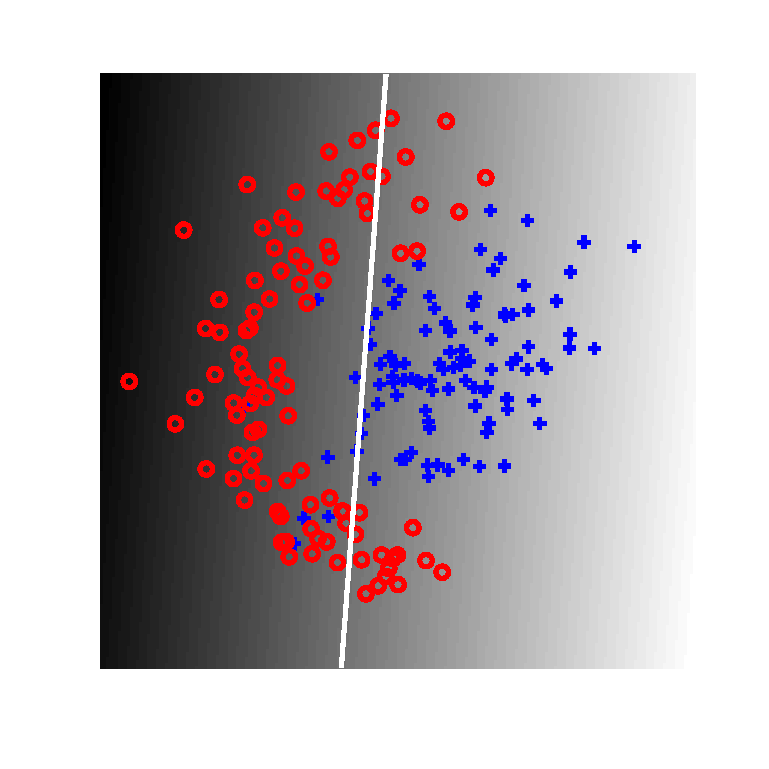
\includegraphics[width=\textwidth]{./lecture6/LinClassification.pdf}
		\caption{Linear classification.}
	\end{subfigure}
	~
	\begin{subfigure}[b]{0.45\textwidth}
		\centering
		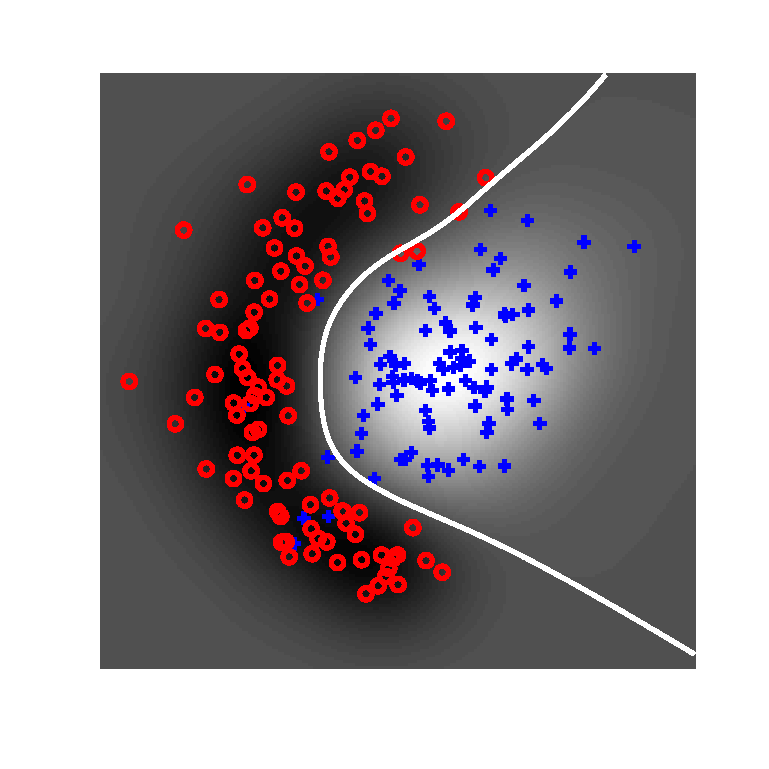
\includegraphics[width=\textwidth]{./lecture6/NonLinClassification.pdf}
		\caption{Non-linear classification.}
	\end{subfigure}
	\caption{A classical dichotomous classification problem where the blue crosses belong to the positive class and the red circles belong to the negative class. We want to find a function which separates the two classes.}
\end{figure}

Of course, linear algorithms can be used together with \emph{nonlinear feature spaces} or \emph{nonlinear basis functions} in order to solve nonlinear classification problems!


\textbf{Linear discriminants separate the space by a hyperplane, and the parameters define its normal vector.} 

\begin{itemize}
\item Decision function: $y(\xx)=\omega^\top \xx + \omega_o$
\item  Classification: \begin{align}
\mbox{if~}y(\xx)>0 & \mbox{~say $\xx$ belongs to class 1}\\
\mbox{if~}y(\xx)<0 & \mbox{~say $\xx$ belongs to class -1}\\
 \end{align}
\item The decision-surface has equation $y(\xx)=0$, and is a hyperplane of dimensionality $D-1$ (codimension).
\item  $\omega$ is the normal vector to the plane, and points into the positive class.
\item  $\omega_o$ determines the location of the decision-surface \\
	   changing $\omega_o$ changes the ratio between FPs and FNs
\item  $|y(\xx)|$ is proproptional to the perpendicular distance to the decision-surface (with factor $1$ if $|| \omega ||=1$).
\item the distance of a data point from the hyperplane reflects the certainty about the class membership.
\end{itemize}


\textbf{Multiple algorithms and methods exist for finding a good $\omega$.} 
\begin{itemize}
\item Mis-classification rate $C(\omega)= \frac{1}{N} \sum_n \overbrace{\delta\left[y(\xx_n) =t_n\right]}^{\delta(x=0) = 1; \; \delta(x \not= 0) = 0}$ (i.e. average number of errors) difficult to optimize over $\omega$, and might have multiple solutions.
	\begin{itemize}
		\item This error function is not continuous and therfore not differentiable	
		\item No convergence if there is no solution with zero errors
		\item Compare: Rosenblatt perceptron. The perceptron learning rule utilizes a 0-1-loss function and is guaranteed to converge in a finite number of steps as long as the data is linearly seperable. It will however not converge for overlapping data.
	\end{itemize}
\item  Many algorithms can be derived by replacing $C$ by another cost-function which can be optimized.
\item  Linear classification algorithms include Least-square classification, Fisher's linear Discriminant, Logistic regression, Support Vector Machines and Rosenblatts' perceptron.
\end{itemize}


\subsection{Least Square Classification}
\textbf{You already know one algorithm for linear classification: least square classification.} 
\begin{itemize}
\item We have to fit the function $y(\xx)= \omega^\top \xx+ \omega_o $ to data.
\item  Simply do a linear regression from $\xx$ to $t$ by minimizing the sum-of-squared errors $\sum_n (y(\xx_n)-t_n)^2$.
\item  $\omega_{reg}=  \left(\sum_n x_n x_n^\top  \right)^{-1} \sum_n x_n t_n$
\item  Q: In what situations might this be a bad idea?
\end{itemize}

\begin{bbbox}{Q: In what situations might this be a bad idea?}
	In the case of a least-squares classification the hyperplane is mainly constrained by data points far away from the decision boundary. However if those data points are not perfectly aligned with the rest of the data points from the same class this can lead to a strong estimation error for the decision boundary as can be seen in figure \ref{fig:least_sq_class} left. A preferable measure contrains the hyperplane based on data points close to the decision boundary and neglects outliers. Compare: Support Vector Machine.
\end{bbbox}

\begin{figure}
	\centering
	\begin{subfigure}[b]{0.45\textwidth}
		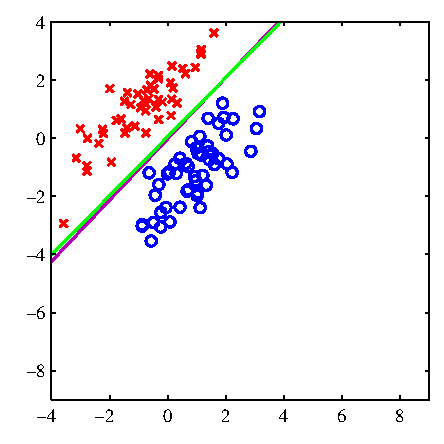
\includegraphics[width=\textwidth]{./lecture6/Figure44a.pdf}
	\end{subfigure}
	~
	\begin{subfigure}[b]{0.45\textwidth}
		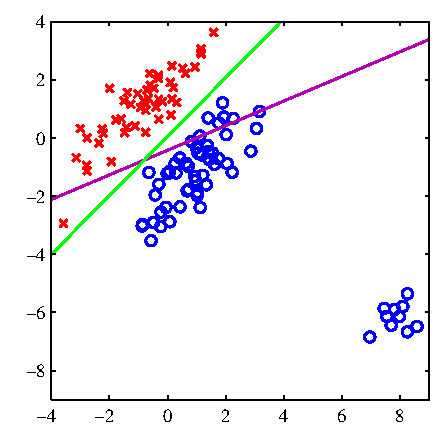
\includegraphics[width=\textwidth]{./lecture6/Figure44b.pdf}
	\end{subfigure}
	\caption{Bishop Figure 4.4}
	\label{fig:least_sq_class}
\end{figure}




\subsection{Fisher's linear discriminant}
\textbf{'Fisher's linear discriminant' is a classical and simple algorithm for linear classification} 


\begin{figure}
	\centering
	\begin{subfigure}[b]{0.45\textwidth}
		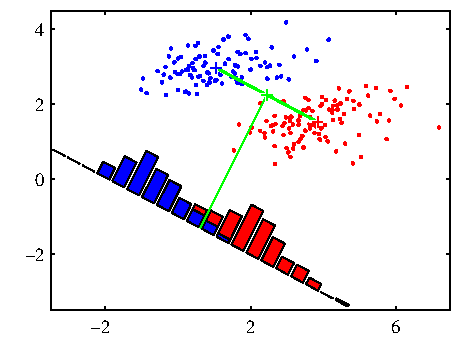
\includegraphics[width=\textwidth]{./lecture6/Figure46a.pdf}
		\caption{Separartion of the projected class means}
	\end{subfigure}
	~
	\begin{subfigure}[b]{0.45\textwidth}
		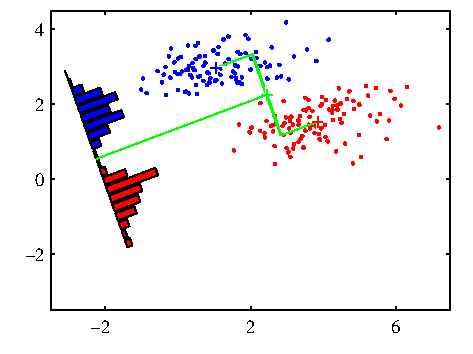
\includegraphics[width=\textwidth]{./lecture6/Figure46b.pdf}
		\caption{Fisher linear discriminant.}
	\end{subfigure}
	\caption{Bishop Figure 4.6}
\end{figure}


\begin{itemize}
\item $\mathbf{m_+}= \frac{1}{N_+}\sum_{n \in C_+} x_n$ \hspace{.5cm} $\mathbf{m_{-}}= \frac{1}{N_-}\sum_{n \in C_{-}} x_n$ 
\item  Maximize projection-distance of class means 
[projected mean/variance: on board]
$\omega_{simple} \propto \mathbf{m}_+-\mathbf{m}_-$ 
\end{itemize}

\begin{bbbox}{Maximize projection-distance of class means. The simple rule.}
	\begin{flalign*}
		&\text{Find } \omega \text{ such that} \\
		&d(m_+,m_-) \text{ is minimized} \\
		&\text{subject to } \|w\| = 1 \\
		&\text{where } d = \left( \omega^{\top} m_+ - \omega^{\top} m_- \right)^2 \\
		&\Rightarrow \omega_{opt} = \alpha \left(m_+ - m_- \right)
	\end{flalign*}
\end{bbbox}

\begin{itemize}
\item  Maximizing distance between means ignores that the projected variances might also be big. 
\item  Fix:  Maximize the ratio of between-class variance to within-class variance ('signal to noise'). Fisher criterion
\begin{align}
	J_\omega = 2\frac{(m_+-m_-)^2}{s_+^2+s_-^2}
\end{align}
[Details and solution: on board]

\begin{bbbox}{Fisher's linear discriminant: Maximize the ratio of between-class variance and within-class variance.}
	\begin{align*}
		\text{Numerator: } N &= d\left( \omega^{\top}m_+, \omega^{\top}m_- \right) \\
		                     &= \left( \omega^{\top} m_+ - \omega^{\top} m_- \right)^2 \\
%		                     &=: (m_+-m_-)^2 \\
%		N &= \left( \omega^{\top} m_+ - \omega^{\top} m_- \right)^2 \\
		  &= \left( \omega^{\top} m_+ - \omega^{\top} m_- \right) \left( \omega^{\top} m_+ - \omega^{\top} m_- \right)^{\top} \\
		  &= \omega^{\top} (m_+-m_-) (m_+-m_-)^{\top} \omega \\
		  &= \omega^{\top} \underbrace{S_B}_{\text{between-class variance}} \omega \\
		S_+^2 &= \mbox{Var}	\left( \omega^{\top} x | x \in C_+ \right) \\
			  &= \omega^{\top} \mbox{Cov}	\left( x | x \in C_+ \right) \omega \\
        S_-^2 &= \omega^{\top} \mbox{Cov}	\underbrace{\left( x | x \in C_- \right)}_{\Sigma_-} \omega \\
        D &= \omega^{\top} \left[ \frac{1}{2} \Sigma_+ + \frac{1}{2} \Sigma_- \right] \omega \\
          &= \omega^{\top} \underbrace{S_W}_{\text{within-class variance}} \omega \\
        J(\omega) &= \frac{N}{D} = \frac{\omega^{\top} S_B \omega}{\omega^{\top} S_W \omega} \\
        \Rightarrow \omega_{opt} \propto S_W^{-1} \left(m_+ - m_- \right)
	\end{align*}
\end{bbbox}

 
$\omega_{lda}= \Sigma_w^{-1} (\mathbf{m}_+-\mathbf{m}_-)$ \\
However Fisher's linear discriminant is still sensitive to outliers.
\end{itemize}

%http://users.informatik.uni-halle.de/~hinnebur/Lehre/BN_seminar_web/bn_05_ag.pdf


\textbf{Aside: The multivariate Gaussian} 
\begin{itemize}
\item Probability density function of $D$ dimensional Gaussian with mean $\mu$ an covariance $\Sigma$: \begin{align}p(x| \mu, \Sigma)&= (2\pi)^{-D/2}|\Sigma|^{-1/2} \exp \left(-\frac{1}{2} (x-\mu)^\top \Sigma^{-1} (x-\mu) \right) \\
 \end{align}
\item  Maximum likelihood estimation of parameters: \begin{align}
\hat\mu= &\frac{1}{N}\sum_n x_n\mbox{~~(empirical mean)}\\ 
\hat \Sigma= &\frac{1}{N} \sum_n x_n x_n^\top- \hat\mu \hat \mu^\top\mbox{~~(empirical covariance)} 
 \end{align}
\end{itemize}


\begin{figure}
	\centering
	\begin{subfigure}[b]{0.3\textwidth}
		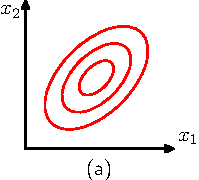
\includegraphics[width=\textwidth]{./lecture6/Figure28a.pdf}
		\caption{Positive correlation.}
	\end{subfigure}
	~
	\begin{subfigure}[b]{0.3\textwidth}
		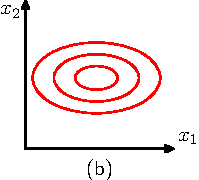
\includegraphics[width=\textwidth]{./lecture6/Figure28b.pdf}
		\caption{Independence but different variances.}
	\end{subfigure}
	~
	\begin{subfigure}[b]{0.3\textwidth}
		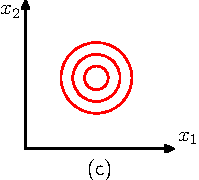
\includegraphics[width=\textwidth]{./lecture6/Figure28c.pdf}
		\caption{Independence and uni-variance.}
	\end{subfigure}
	\caption{Multivariate Gaussians with different covariance matrices. Bishop Figure 2.8}
\end{figure}

\textbf{A (super brief) primer on covariance matrices. (more details/intuition in second half of course?)} 

\begin{figure}
	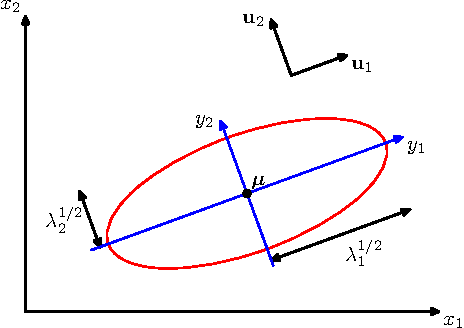
\includegraphics[width=.45\textwidth]{./lecture6/Figure27.pdf}
	\caption{Bishop Figure 2.7}
\end{figure}

\begin{itemize}
	\item  Covariance matrices are symmetric.
	\item  Diagonal entries: variances along coordinate-axes
	\item  Eigenvectors: principal axes of ellipsoid
	\item Eigenvalues:  variances along eigen-vectors
	\item Eigenvector with maximal/minimal eigen-value: Direction of maximal/minimal variance 
	\item  Covariance matrices are `positive definite', i.e. all their eigenvalues are non-negative.
	\item  Most of this can be derived from $a^\top \mbox{Cov}(X) a= \mbox{Var}(a^\top X)$
\end{itemize}

\subsection{A generative model: Class-conditional Gaussians}
\textbf{A tale of two Gaussian: We can use a probablistic model of the data for classification} 

\begin{figure}
	\centering
	\begin{subfigure}[b]{0.45\textwidth}
		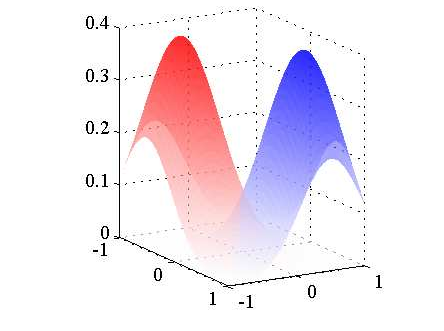
\includegraphics[width=\textwidth]{./lecture6/Figure410a.pdf}
	\end{subfigure}
	~
	\begin{subfigure}[b]{0.45\textwidth}
		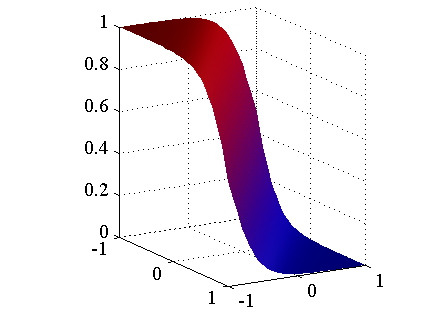
\includegraphics[width=\textwidth]{./lecture6/Figure410b.pdf}
	\end{subfigure}
	\caption{Bishop 4.10}
\end{figure}


\begin{itemize}
	\item Suppose that each of the two classes is modelled by a Gaussian: $x | x \in C_+ \sim \mathcal{N}\left(\mu_+, \Sigma_+\right)$, $x | x \in C_- \sim \mathcal{N}\left(\mu_-, \Sigma_-\right)$, 
	\item ~[On board] Calculation of posterior class probabilities and decision criterion
	\item  If we assume $\Sigma_+=\Sigma_-$, we get $\omega_{gauss} \propto \Sigma_+^{-1} (\mathbf{m}_+-\mathbf{m}_-)$
	\item Note: We take the $t_n$ as given and built a model of $x_n | t_n$, contrast with linear regression, where we took $x_n$ as given and modelled $t_n |x_n$.
\end{itemize}

\begin{bbbox}{Probabilistic generative model: Gaussians}
We assume that data from each of the two classes is normally distributed  such that: \\
	\begin{flalign*}
	& P(x|t=1) = \mathcal{N}\left( x| \mu_+,\Sigma_+ \right) &\\
	& P(x|t=-1) = \mathcal{N}\left( x| \mu_-,\Sigma_- \right) &\\
	\end{flalign*}

If we know the prior probabilities $\pi$ for observing data from any of the two classes we can caculate the posterior probability of a data point belonging to each of the classes. This is by simply utilizing Bayes' theorem. \\
	\begin{flalign*}
	& P(t=1|x) = \frac{1}{Z} P(x|t=1) \underbrace{P(t=1)}_{\pi_+} = \frac{\pi_+}{Z} P(x|t=1) &\\
	& \text{where} &\\
	& Z = \pi_+ P(x | t = 1) + \pi_{-} P(x | t = -1) \text{ is a normalization constant} &\\
	& \text{and} &\\
	& P(t = 1 | x) + P(t = -1|x) = 1	&\\
	\end{flalign*}
	
We now use the log-odds to find the decision boundary for our classification problem. We assign data point $x$ to the positive class if $d(x) > 0$ and we will assign it to the negative class otherwise: \\
	\begin{flalign*}
		d(x) &=  \log \left[ \frac{P(t=1|x)}{P(t=-1|x)}\right] \\
		     &= C - \frac{1}{2} \left(x-\mu_+\right)^{\top} \Sigma_+^{-1} \left(x-\mu_+\right) \\
		     	 &\qquad {} + \frac{1}{2} \left(x-\mu_-\right)^{\top} \Sigma_-^{-1} \left(x-\mu_-\right) \\
		\textbf{Assume } \Sigma_+ = \Sigma_- = \Sigma  \\
		     &= C - \frac{1}{2} x^{\top} \Sigma^{-1} x + \frac{1}{2} \mu_+^{\top} \Sigma^{-1} x + \frac{1}{2} x^{\top} \Sigma^{-1} \mu_+ - \frac{1}{2} \mu_+^{\top} \Sigma^{-1} \mu_+ \\
		        &\qquad {} + \frac{1}{2} x^{\top} \Sigma^{-1} x - \frac{1}{2} \mu_-^{\top} \Sigma^{-1} x -\frac{1}{2} x^{\top} \Sigma^{-1} \mu_- + \frac{1}{2} \mu_-^{\top} \Sigma^{-1} \mu_- \\
		     &= C_2 + \mu_+^{\top} \Sigma^{-1} x - \mu_-^{\top} \Sigma^{-1} x \\
		     &= C_2 + \left( \mu_+ - \mu_- \right)^{\top} \Sigma^{-1} x \\
		     &= C_2 + \left[ \Sigma^{-1} \left( \mu_+ - \mu_- \right) \right]^{\top} x \\		     
		     &= \omega_0 + \omega^{\top}x
	\end{flalign*}
If we compare this result with our results for FDA and linear regression for classification we realize that all three approach lead to equivalent decision boundaries.
\end{bbbox}

\textbf{This approach directly generalizes to classification with unequal covariances and multi-class classification.}

\begin{figure}
	\centering
	\begin{subfigure}[b]{0.45\textwidth}
		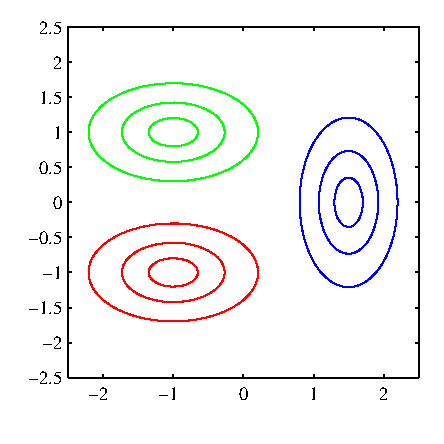
\includegraphics[width=\textwidth]{./lecture6/Figure411a.pdf}
	\end{subfigure}
	~
	\begin{subfigure}[b]{0.45\textwidth}
		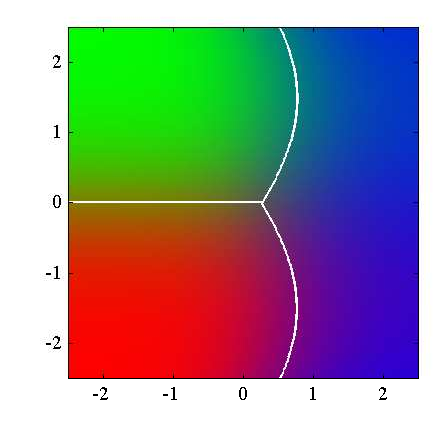
\includegraphics[width=\textwidth]{./lecture6/Figure411b.pdf}
	\end{subfigure}
	\caption{Bishop 4.11}
\end{figure}

\begin{itemize}
\item Quadratic discriminant analysis: $\Sigma_+ \neq \Sigma_o$, decisison boundary is of form $y(\xx) = \xx^\top A \xx+\omega^\top \xx +\omega_o$
\item Multi-class: Assign each data-point to class with highest posterior probability (or calculate best assignment from cost-function). 
\end{itemize}

\textbf{A simple nonlinear classifier can be constructed from kernel density estimates of the probability densities.}

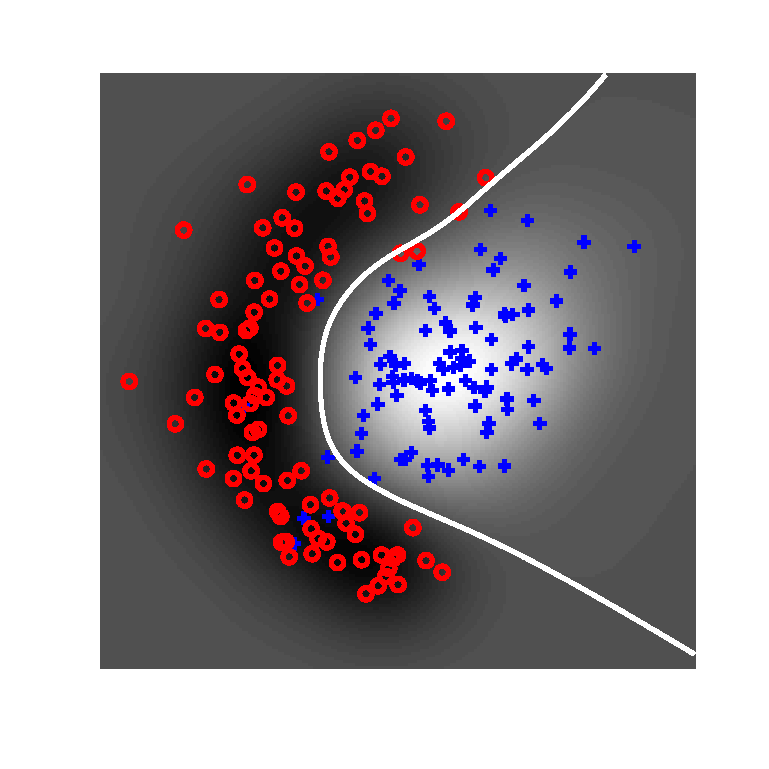
\includegraphics[width=\textwidth]{./lecture6/NonLinClassification.pdf}
\begin{itemize}
	\item Idea: Once we have an estimate of the class-conditional densities $P(x| t=\pm 1)$, we can construct a rule from $d(x)=P(x| t=+ 1)-P(x| t=- 1)$.
	\item  Use \emph{kernel density estimation} to estimate  $P(x| t=\pm 1)$, i.e. place a `Gaussian bump' on each data-point:
	\begin{align}
		P(x| t=1) =\frac{1}{Z}\sum_{n_+} \exp\left( \frac{x-x_n}{\sigma}\right)^2
	\end{align}
\end{itemize}

This leads to a classifier of the form
\begin{align}
	d(x)= \sum_{n} \alpha  t_n \exp\left( \frac{x-x_n}{\sigma}\right)^2
\end{align}

\emph{Support vector machine with radial basis functions} has decision rule 
\begin{align}
	d(x)=\sum_{n}  \alpha_n \exp\left( \frac{x-x_n}{\sigma}\right)^2
\end{align}





\subsection{One for the price of three.} 
\begin{itemize}
	\item Today, you learned about three different algorithms for binary classification with linear decision rules. 
	\item  One was based on a hack, the second one on a plausible (but ad-hoc) criterion, and the third one an a probababilistic model of the data.
	\item  All three algorithms are equivalent.
	\item  We showed that the Fisher discriminant and the probabilistic model based on two Gaussians have the same  decision criterion. In fact, it can be shown that linear regression has the same weights (Bishop 4.1.5)
%\item  The moral: Great motivations are great, but the actual algorithm matters, and it is important to check connections with other algorithms.
	\item The third motivation had immediate extensions to nonlinear algorithms and multi-class classification, and posterior probabilities.
	\item  Next week, we will learn an algorithm which actually is different, and usually better than the ones discussed today.
\end{itemize}

